\documentclass[conference]{IEEEtran}
\IEEEoverridecommandlockouts
% The preceding line is only needed to identify funding in the first footnote. If that is unneeded, please comment it out.
\usepackage{cite}
\usepackage{amsmath,amssymb,amsfonts}
\usepackage{algorithmic}
\usepackage{graphicx}
\usepackage{textcomp}
\usepackage{xcolor}
\def\BibTeX{{\rm B\kern-.05em{\sc i\kern-.025em b}\kern-.08em
    T\kern-.1667em\lower.7ex\hbox{E}\kern-.125emX}}
\begin{document}

\title{Performance measurements for Differentiated Services in IPv4 and IPv6\\
{\footnotesize \textsuperscript{}}
\thanks{Identify applicable funding agency here. If none, delete this.}
}

\author{\IEEEauthorblockN{1\textsuperscript{st} Nils Rodday}
\IEEEauthorblockA{\textit{Universit{\"a}t der Bundeswehr M{\"u}nchen \&} \\
\textit{University of Twente}\\
Neubiberg, Germany \\
nils.rodday@unibw.de}
\and
\IEEEauthorblockN{2\textsuperscript{nd} Klement Streit}
\IEEEauthorblockA{\textit{CODE Research Institute} \\
\textit{Universit{\"a}t der Bundeswehr M{\"u}nchen} \\
Neubiberg, Germany \\
klement.streit@unibw.de}
\and
\IEEEauthorblockN{3\textsuperscript{rd} Gabi Dreo Rodosek}
\IEEEauthorblockA{\textit{CODE Research Institute} \\
\textit{Universit{\"a}t der Bundeswehr M{\"u}nchen} \\
Neubiberg, Germany \\
gabi.dreo@unibw.de}
\and
\IEEEauthorblockN{4\textsuperscript{th} Aiko Pras}
\IEEEauthorblockA{\textit{DACS Research Group} \\
\textit{University of Twente}\\
Enschede, Netherlands \\
aiko.pras@utwente.nl}
}

\maketitle

\begin{abstract}



\end{abstract}

\begin{IEEEkeywords}
Measurement campaign, Quality of Service, QoS, TOS field, DSCP
\end{IEEEkeywords}

\section{Introduction}
The Internet only provides best effort services to its connected participants and does not provide delivery or performance guarantees. However, since the very beginning of the standardization of the IP protocol, Quality of Service was recognized as an important topic. The Type of Service (TOS) and Traffic Class fields were included in the IPv4 and IPv6 headers, respectively,  consisting of 8 Bits which are reserved for the use of QoS meachanisms, allowing packets to get prioritized on their way through the routing infrastructure. In IPv6 an additional Flow Label was added to the header with 20 Bits. But how efficient is this mechanism and does its use indeed provide greater performance with lower latency and faster deliver of packets? And how many routers are supporting these QoS mechanism and honor TOS bits set in the IP header? This research aims to answer those questions by performing a large scale measurement campaign. We look at the different priority categories and compare their support in routers in IPv4 and IPv6. \\

In IPv4 the QoS mechanism in the IP header was called the TOS field, in IPv6 it was called Traffic Class (TC). RFC 2474 attempts to rename the TOS octet of the IPV4 header, and Traffic Class octet of the IPV6 header, respectively, to the Differentiated Services (DS) field \cite{b1}. The DS field takes up 6 Bits, leaving 2 Bits as Currently Unused (CU) bits. Figure \ref{fig:QoS-value} illustrates the separation. Multiple categories called the Differentiated Services Code Point (DSCP) were defined and encoded in the DS field to represent the priority of a packet, which can be found in Table \ref{tab1:DSCP-categories}. In order to support legacy systems that do not already implement the newest standard, the first 3 Bits in the Class Selector range are mapping to the Precedence Bits of the previous interpretation. Therefore, even systems following the old standards are still able to understand the QoS that is desired by the sender. \\



\begin{figure}
\centerline{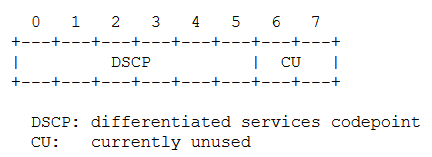
\includegraphics{figures/QoS_field.png}}
\caption{DSCP and CU}
\label{fig:QoS-value}
\end{figure}


\begin{table}[htbp]
\caption{QoS mapping in the IP header}
\begin{center}
\begin{tabular}{|c|c|c|c|c|}
\hline
\textbf{DSCP}& \textbf{Binary} & \textbf{IP Precedence} & \textbf{AF class} & \textbf{Drop prob.} \\
\hline
CS0 & 000 000 & Routine & Best effort & test  \\
CS1 & 001 000 & Priority & AF11/AF12/AF13 & test \\
CS2 & 010 000 & Immediate & AF21/AF22/AF23 & test \\
CS3 & 011 000 & Flash & AF31/AF32/AF33 & test \\
CS4 & 100 000 & Flash Override & AF41/AF42/AF43 & test \\
CS5 & 101 000 & Critical & test & test \\
CS6 & 110 000 & Internet & test & test \\
CS7 & 111 000 & Network & test & test \\

\hline
\multicolumn{4}{l}{$^{\mathrm{a}}$Sample of a Table footnote.}
\end{tabular}
\label{tab1:DSCP-categories}
\end{center}
\end{table}

\section{Related Work}



\section{Research Questions}

We defined the following research questions:

\begin{enumerate}

\item How much benefit in performance do we gain by using the different QoS mechanisms of the DS field in the current Internet infrastructure in IPv4 and IPv6?
\item What share of routers is currently supporting QoS and to which extent?
\item Since there are ambiguties in what different RFCs specify for the use of those 8 bits, what share of routers is following which convention?
\item Are certain autonomous systems (AS) providing better support of QoS than others?

\end{enumerate}

\section{Methodology}

In order to answer the previously defined research questions, we will perform a large scale measurement campaign using the infrastructure of PlanetLab. PlanetLab has the advantage to provide several thousands of vantage points (VP) all over the world in different networks. It gives us the opportunity to test the different categories of QoS parameters and discover differences that are based on routes taken depeding on the geolocation of sender and recipient.

\subsection{Measurement Architecture}


\subsection{Types of Measurements}

We plan to perform the following measurements:






\section*{Acknowledgment}

We thank xyz.

\section*{References}


\begin{thebibliography}{00}
\bibitem{b1} D. Grossman, ``RFC3260,'' IETF, Network Working Group, 2002.


\bibitem{b2} J. Clerk Maxwell, A Treatise on Electricity and Magnetism, 3rd ed., vol. 2. Oxford: Clarendon, 1892, pp.68--73.
\bibitem{b3} I. S. Jacobs and C. P. Bean, ``Fine particles, thin films and exchange anisotropy,'' in Magnetism, vol. III, G. T. Rado and H. Suhl, Eds. New York: Academic, 1963, pp. 271--350.
\bibitem{b4} K. Elissa, ``Title of paper if known,'' unpublished.
\bibitem{b5} R. Nicole, ``Title of paper with only first word capitalized,'' J. Name Stand. Abbrev., in press.
\bibitem{b6} Y. Yorozu, M. Hirano, K. Oka, and Y. Tagawa, ``Electron spectroscopy studies on magneto-optical media and plastic substrate interface,'' IEEE Transl. J. Magn. Japan, vol. 2, pp. 740--741, August 1987 [Digests 9th Annual Conf. Magnetics Japan, p. 301, 1982].
\bibitem{b7} M. Young, The Technical Writer's Handbook. Mill Valley, CA: University Science, 1989.
\end{thebibliography}
\vspace{12pt}
\color{red}
IEEE conference templates contain guidance text for composing and formatting conference papers. Please ensure that all template text is removed from your conference paper prior to submission to the conference. Failure to remove the template text from your paper may result in your paper not being published.

\end{document}
